% Options for packages loaded elsewhere
\PassOptionsToPackage{unicode}{hyperref}
\PassOptionsToPackage{hyphens}{url}
%
\documentclass[
  ignorenonframetext,
]{beamer}
\usepackage{pgfpages}
\setbeamertemplate{caption}[numbered]
\setbeamertemplate{caption label separator}{: }
\setbeamercolor{caption name}{fg=normal text.fg}
\beamertemplatenavigationsymbolsempty
% Prevent slide breaks in the middle of a paragraph
\widowpenalties 1 10000
\raggedbottom
\setbeamertemplate{part page}{
  \centering
  \begin{beamercolorbox}[sep=16pt,center]{part title}
    \usebeamerfont{part title}\insertpart\par
  \end{beamercolorbox}
}
\setbeamertemplate{section page}{
  \centering
  \begin{beamercolorbox}[sep=12pt,center]{part title}
    \usebeamerfont{section title}\insertsection\par
  \end{beamercolorbox}
}
\setbeamertemplate{subsection page}{
  \centering
  \begin{beamercolorbox}[sep=8pt,center]{part title}
    \usebeamerfont{subsection title}\insertsubsection\par
  \end{beamercolorbox}
}
\AtBeginPart{
  \frame{\partpage}
}
\AtBeginSection{
  \ifbibliography
  \else
    \frame{\sectionpage}
  \fi
}
\AtBeginSubsection{
  \frame{\subsectionpage}
}

\usepackage{amsmath,amssymb}
\usepackage{lmodern}
\usepackage{iftex}
\ifPDFTeX
  \usepackage[T1]{fontenc}
  \usepackage[utf8]{inputenc}
  \usepackage{textcomp} % provide euro and other symbols
\else % if luatex or xetex
  \usepackage{unicode-math}
  \defaultfontfeatures{Scale=MatchLowercase}
  \defaultfontfeatures[\rmfamily]{Ligatures=TeX,Scale=1}
\fi
\usetheme[]{sky}
% Use upquote if available, for straight quotes in verbatim environments
\IfFileExists{upquote.sty}{\usepackage{upquote}}{}
\IfFileExists{microtype.sty}{% use microtype if available
  \usepackage[]{microtype}
  \UseMicrotypeSet[protrusion]{basicmath} % disable protrusion for tt fonts
}{}
\makeatletter
\@ifundefined{KOMAClassName}{% if non-KOMA class
  \IfFileExists{parskip.sty}{%
    \usepackage{parskip}
  }{% else
    \setlength{\parindent}{0pt}
    \setlength{\parskip}{6pt plus 2pt minus 1pt}}
}{% if KOMA class
  \KOMAoptions{parskip=half}}
\makeatother
\usepackage{xcolor}
\newif\ifbibliography
\setlength{\emergencystretch}{3em} % prevent overfull lines
\setcounter{secnumdepth}{-\maxdimen} % remove section numbering

\usepackage{color}
\usepackage{fancyvrb}
\newcommand{\VerbBar}{|}
\newcommand{\VERB}{\Verb[commandchars=\\\{\}]}
\DefineVerbatimEnvironment{Highlighting}{Verbatim}{commandchars=\\\{\}}
% Add ',fontsize=\small' for more characters per line
\usepackage{framed}
\definecolor{shadecolor}{RGB}{241,243,245}
\newenvironment{Shaded}{\begin{snugshade}}{\end{snugshade}}
\newcommand{\AlertTok}[1]{\textcolor[rgb]{0.68,0.00,0.00}{#1}}
\newcommand{\AnnotationTok}[1]{\textcolor[rgb]{0.37,0.37,0.37}{#1}}
\newcommand{\AttributeTok}[1]{\textcolor[rgb]{0.40,0.45,0.13}{#1}}
\newcommand{\BaseNTok}[1]{\textcolor[rgb]{0.68,0.00,0.00}{#1}}
\newcommand{\BuiltInTok}[1]{\textcolor[rgb]{0.00,0.23,0.31}{#1}}
\newcommand{\CharTok}[1]{\textcolor[rgb]{0.13,0.47,0.30}{#1}}
\newcommand{\CommentTok}[1]{\textcolor[rgb]{0.37,0.37,0.37}{#1}}
\newcommand{\CommentVarTok}[1]{\textcolor[rgb]{0.37,0.37,0.37}{\textit{#1}}}
\newcommand{\ConstantTok}[1]{\textcolor[rgb]{0.56,0.35,0.01}{#1}}
\newcommand{\ControlFlowTok}[1]{\textcolor[rgb]{0.00,0.23,0.31}{#1}}
\newcommand{\DataTypeTok}[1]{\textcolor[rgb]{0.68,0.00,0.00}{#1}}
\newcommand{\DecValTok}[1]{\textcolor[rgb]{0.68,0.00,0.00}{#1}}
\newcommand{\DocumentationTok}[1]{\textcolor[rgb]{0.37,0.37,0.37}{\textit{#1}}}
\newcommand{\ErrorTok}[1]{\textcolor[rgb]{0.68,0.00,0.00}{#1}}
\newcommand{\ExtensionTok}[1]{\textcolor[rgb]{0.00,0.23,0.31}{#1}}
\newcommand{\FloatTok}[1]{\textcolor[rgb]{0.68,0.00,0.00}{#1}}
\newcommand{\FunctionTok}[1]{\textcolor[rgb]{0.28,0.35,0.67}{#1}}
\newcommand{\ImportTok}[1]{\textcolor[rgb]{0.00,0.46,0.62}{#1}}
\newcommand{\InformationTok}[1]{\textcolor[rgb]{0.37,0.37,0.37}{#1}}
\newcommand{\KeywordTok}[1]{\textcolor[rgb]{0.00,0.23,0.31}{#1}}
\newcommand{\NormalTok}[1]{\textcolor[rgb]{0.00,0.23,0.31}{#1}}
\newcommand{\OperatorTok}[1]{\textcolor[rgb]{0.37,0.37,0.37}{#1}}
\newcommand{\OtherTok}[1]{\textcolor[rgb]{0.00,0.23,0.31}{#1}}
\newcommand{\PreprocessorTok}[1]{\textcolor[rgb]{0.68,0.00,0.00}{#1}}
\newcommand{\RegionMarkerTok}[1]{\textcolor[rgb]{0.00,0.23,0.31}{#1}}
\newcommand{\SpecialCharTok}[1]{\textcolor[rgb]{0.37,0.37,0.37}{#1}}
\newcommand{\SpecialStringTok}[1]{\textcolor[rgb]{0.13,0.47,0.30}{#1}}
\newcommand{\StringTok}[1]{\textcolor[rgb]{0.13,0.47,0.30}{#1}}
\newcommand{\VariableTok}[1]{\textcolor[rgb]{0.07,0.07,0.07}{#1}}
\newcommand{\VerbatimStringTok}[1]{\textcolor[rgb]{0.13,0.47,0.30}{#1}}
\newcommand{\WarningTok}[1]{\textcolor[rgb]{0.37,0.37,0.37}{\textit{#1}}}

\providecommand{\tightlist}{%
  \setlength{\itemsep}{0pt}\setlength{\parskip}{0pt}}\usepackage{longtable,booktabs,array}
\usepackage{calc} % for calculating minipage widths
\usepackage{caption}
% Make caption package work with longtable
\makeatletter
\def\fnum@table{\tablename~\thetable}
\makeatother
\usepackage{graphicx}
\makeatletter
\def\maxwidth{\ifdim\Gin@nat@width>\linewidth\linewidth\else\Gin@nat@width\fi}
\def\maxheight{\ifdim\Gin@nat@height>\textheight\textheight\else\Gin@nat@height\fi}
\makeatother
% Scale images if necessary, so that they will not overflow the page
% margins by default, and it is still possible to overwrite the defaults
% using explicit options in \includegraphics[width, height, ...]{}
\setkeys{Gin}{width=\maxwidth,height=\maxheight,keepaspectratio}
% Set default figure placement to htbp
\makeatletter
\def\fps@figure{htbp}
\makeatother

\usepackage{booktabs}
\usepackage{longtable}
\usepackage{array}
\usepackage{multirow}
\usepackage{wrapfig}
\usepackage{float}
\usepackage{colortbl}
\usepackage{pdflscape}
\usepackage{tabu}
\usepackage{threeparttable}
\usepackage{threeparttablex}
\usepackage[normalem]{ulem}
\usepackage{makecell}
\usepackage{xcolor}
\makeatletter
\makeatother
\makeatletter
\makeatother
\makeatletter
\@ifpackageloaded{caption}{}{\usepackage{caption}}
\AtBeginDocument{%
\ifdefined\contentsname
  \renewcommand*\contentsname{Table of contents}
\else
  \newcommand\contentsname{Table of contents}
\fi
\ifdefined\listfigurename
  \renewcommand*\listfigurename{List of Figures}
\else
  \newcommand\listfigurename{List of Figures}
\fi
\ifdefined\listtablename
  \renewcommand*\listtablename{List of Tables}
\else
  \newcommand\listtablename{List of Tables}
\fi
\ifdefined\figurename
  \renewcommand*\figurename{Figure}
\else
  \newcommand\figurename{Figure}
\fi
\ifdefined\tablename
  \renewcommand*\tablename{Table}
\else
  \newcommand\tablename{Table}
\fi
}
\@ifpackageloaded{float}{}{\usepackage{float}}
\floatstyle{ruled}
\@ifundefined{c@chapter}{\newfloat{codelisting}{h}{lop}}{\newfloat{codelisting}{h}{lop}[chapter]}
\floatname{codelisting}{Listing}
\newcommand*\listoflistings{\listof{codelisting}{List of Listings}}
\makeatother
\makeatletter
\@ifpackageloaded{caption}{}{\usepackage{caption}}
\@ifpackageloaded{subcaption}{}{\usepackage{subcaption}}
\makeatother
\makeatletter
\@ifpackageloaded{tcolorbox}{}{\usepackage[many]{tcolorbox}}
\makeatother
\makeatletter
\@ifundefined{shadecolor}{\definecolor{shadecolor}{rgb}{.97, .97, .97}}
\makeatother
\makeatletter
\makeatother
\ifLuaTeX
  \usepackage{selnolig}  % disable illegal ligatures
\fi
\IfFileExists{bookmark.sty}{\usepackage{bookmark}}{\usepackage{hyperref}}
\IfFileExists{xurl.sty}{\usepackage{xurl}}{} % add URL line breaks if available
\urlstyle{same} % disable monospaced font for URLs
\hypersetup{
  pdftitle={Gendered Journeys to Mixed Unions},
  pdfauthor={Dr.~Marion Lieutaud},
  hidelinks,
  pdfcreator={LaTeX via pandoc}}

\title{Gendered Journeys to Mixed Unions}
\subtitle{BSPS 2022 - Migration Strand}
\author{Dr.~Marion Lieutaud}
\date{}
\institute{London School of Economics, Department of Methodology,
Understanding Society research fellow}
\logo{
\includegraphics{graphics/LSE logo.png}}

\begin{document}
\frame{\titlepage}
\ifdefined\Shaded\renewenvironment{Shaded}{\begin{tcolorbox}[interior hidden, frame hidden, enhanced, borderline west={3pt}{0pt}{shadecolor}, breakable, boxrule=0pt, sharp corners]}{\end{tcolorbox}}\fi

\begin{frame}{Abstract}
\protect\hypertarget{abstract}{}
\note{\emph{Speaker notes go here}

\begin{itemize}
\item
  to enable presentor mode: press `S' key
\item
  to zoom into one part of the slide, press `option' key and click on
  that part
\end{itemize}}

Migrant-native intermarriage is a well-researched topic (Kulu and
Hannemann 2016; Safi 2010) and a cornerstone of theories of
assimilation. However, the gendered dynamics connecting migration and
mixing are at best peripherally mentioned in most quantitative
enquiries. Yet analyses of gendered outcomes of migration have noted the
contrast between the economic and work benefits of intermarriage for
migrant men (very beneficial) and for migrant women (not beneficial)
(Basu 2015; Lieutaud 2021). This could well be explained by more or less
disempowering `journeys' to mixing (e.g.~marriage migrants or `trailing
spouses' vs.~independent `pioneer' migrant (Amparo González-Ferrer et
al.~2018)). This paper investigates the life-course and legal
circumstances of migration which form the backdrop to the formation of a
mixed union, and whether they differ between migrant women and migrant
men. Drawing on survey data from Understanding Society (UK, 2009-) and
Trajectoires et Origines (France, 2008-2009, 2019-2020), I employ
sequence analysis to build a typology of migration journeys (see Castro
Torres 2020; Kulu and Mikolai 2021). I find that couple-forming
migration is a frequent feature of mixed unions involving migrant women,
indicating scenarios where they either followed their partner
immediately after starting the relationship, or were only just arrived.
Migrant men in mixed unions, in contrast, were long there by the time
when they formed a mixed union. Mixed unions in France are also overall
more likely to involve child migrants, which could be connected to
slightly different policies around bringing dependents, and the
importance of school socialization in the French context.

\begin{block}{Introduction}
\protect\hypertarget{introduction}{}
\begin{itemize}
\tightlist
\item
  Bullet 1
\item
  Bullet 2
\item
  Bullet 3
\end{itemize}
\end{block}

\begin{block}{Literature review}
\protect\hypertarget{literature-review}{}
\begin{itemize}
\tightlist
\item
  Intermarriage and assimilation For more details on authoring R
  presentations please visit
  \url{https://support.rstudio.com/hc/en-us/articles/200486468}.
\item
  classics on assimilation: find sections on mixing (Gordon 1964, Alba
  \& Nee, also possibly Porthes \& Zhou for segmented assimilation).
  Look into Safi's \emph{Migration and Inequality}, also Muttarak (2010)
  and Kalmijn
\item
  Gonzales-Ferrer
\item
  Basu
\end{itemize}

\emph{Previous research has framed intermarriage between immigrants and
natives as an indicator of the social distance between groups as well as
a process by which it is bridged. Much of this work focuses on the
demographic structures that provide opportunities and constraints for
exogamous unions (Qian and Lichter, 2001, Qian and Lichter, 2007,
Sassler, 2005) as well as the peer- and family-level influences on
partner choice (De Valk and Liefbroer, 2007, Kalmijn and van Tubergen,
2010). In this paper we add to this literature by examining how the
timing of union formation and marriage is connected to partner choice.}
(Soehl \& Yahirunn, 2011)

See also `Mixed marriages between immigrants and natives in Spain: The
gendered effect of marriage market constraints' (Gonzales-Ferrer
\emph{et al.} 2018)

\begin{itemize}
\tightlist
\item
  The consequences of intermarriage

  \begin{itemize}
  \tightlist
  \item
    labour market performance (Meng \& Gregory 2005, Furtado \&
    Theadoropoulos 2010)
  \item
    the intermarriage `premium': only for migrant men (Nystedt \& Dribe
    2015 - Sweden; Basu 2015; Nottmeyer 2014 on paid and unpaid labour)
  \end{itemize}
\end{itemize}

On gendered processes of ethnic intermarriage (Sassler 2005) (Women's
exogamy being more constrained in the US)
\end{block}

\begin{block}{research question}
\protect\hypertarget{research-question}{}
\end{block}
\end{frame}

\begin{frame}[fragile]{Data and methods}
\protect\hypertarget{data-and-methods}{}
\begin{block}{Data}
\protect\hypertarget{data}{}
UKLHS (2009-) and Trajectoires et Origines (2008-2099)

\begin{center}
\footnotesize
\begin{tabular}{lc}
  \hline
 \textbf{Sub-samples (cumulative criteria)} & \textbf{N} \\ 
  \hline
  UKLHS individual survey respondents (w2) & 54,565 \\ 
  - in cohabiting relationships & 34,281 \\
  - both partners were full survey respondents & 27,058 \\
  - man-woman relationships & 26,826     \\ 
  - both partners of working age (18-60) & 18,200 \\
  - exc. key missing values* & 17,286 \\
  - with individual partnership history data & 15,678 \\
  - migrant respondents only & 2623 \\
 \hline
\end{tabular}
\end{center}

\scriptsize\{* Key missing values refer to missing values for migration
background (whether UK-born) and for couple type.\}

\begin{Shaded}
\begin{Highlighting}[]
\FunctionTok{library}\NormalTok{(kableExtra)}
\FunctionTok{kable}\NormalTok{(}\FunctionTok{summary}\NormalTok{(cars))}
\end{Highlighting}
\end{Shaded}

\begin{tabular}{l|l|l}
\hline
  &     speed &      dist\\
\hline
 & Min.   : 4.0 & Min.   :  2.00\\
\hline
 & 1st Qu.:12.0 & 1st Qu.: 26.00\\
\hline
 & Median :15.0 & Median : 36.00\\
\hline
 & Mean   :15.4 & Mean   : 42.98\\
\hline
 & 3rd Qu.:19.0 & 3rd Qu.: 56.00\\
\hline
 & Max.   :25.0 & Max.   :120.00\\
\hline
\end{tabular}

\note{If we add: ``\#\textbar{} output-location: slide'' at the
beginning of the code chunk, it displays results in the next slide}
\end{block}

\begin{block}{Methods}
\protect\hypertarget{methods}{}
\begin{block}{Sequence analysis}
\protect\hypertarget{sequence-analysis}{}
\end{block}

\begin{block}{Linear and logistic regression models}
\protect\hypertarget{linear-and-logistic-regression-models}{}
\end{block}

\begin{block}{R Packages}
\protect\hypertarget{r-packages}{}
\end{block}

\begin{block}{Wrangling}
\protect\hypertarget{wrangling}{}
\note{Distribution of working time not possible with TeO. Distribution
of income: - not possible because no indicator of partner's income. -
however, there is information on the household's income, and ego's
income. Could work (to a point, and only when looking only at ego=women.
or ego=migrant)}
\end{block}

\begin{block}{Graphical elements}
\protect\hypertarget{graphical-elements}{}
\end{block}

\begin{block}{Survey-weighting}
\protect\hypertarget{survey-weighting}{}
The survey-weighted analyses exclude individuals with missing values
for: - gender-specialisation index (this may be a problem) - cpl
variable (this is legit)
\end{block}
\end{block}
\end{frame}

\begin{frame}{Results}
\protect\hypertarget{results}{}
\begin{block}{barplots: gender division of labour by cpl types}
\protect\hypertarget{barplots-gender-division-of-labour-by-cpl-types}{}
\end{block}

\begin{block}{}
\protect\hypertarget{section}{}
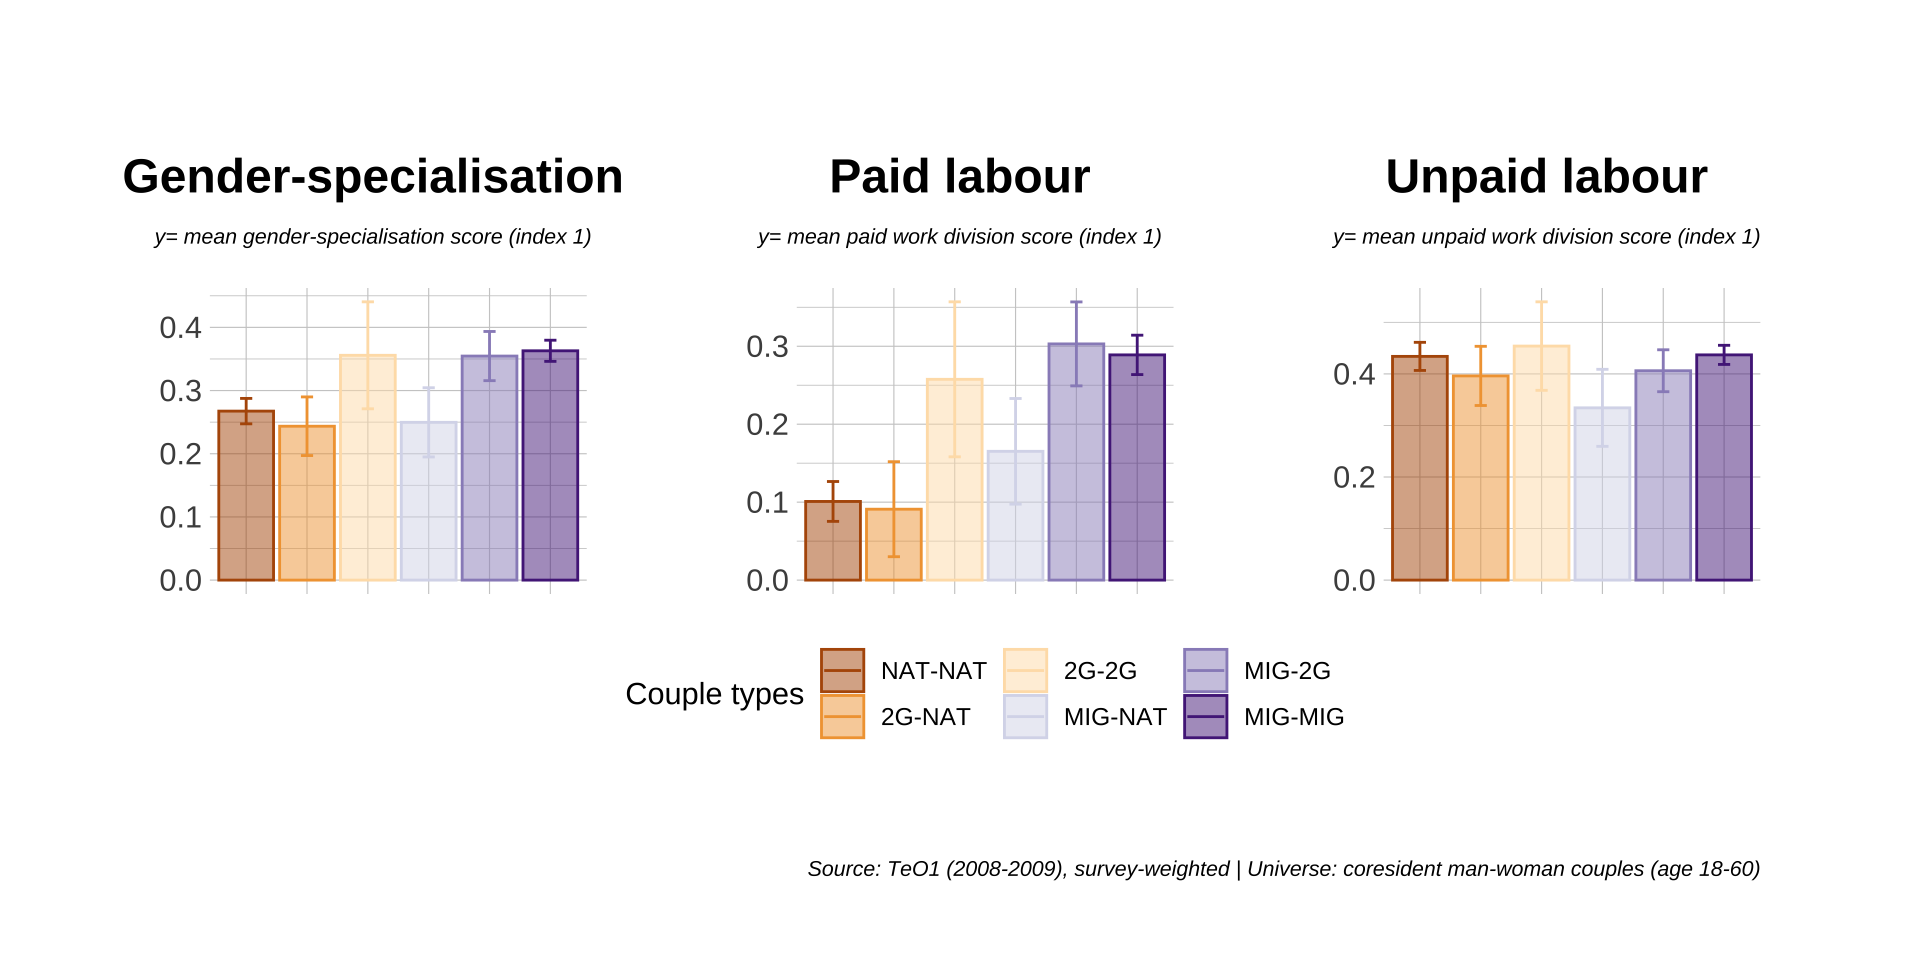
\includegraphics{BSPS-2022-mixed-unions_files/figure-beamer/barplot_gdrspecFR-1.pdf}
\end{block}

\begin{block}{}
\protect\hypertarget{section-1}{}
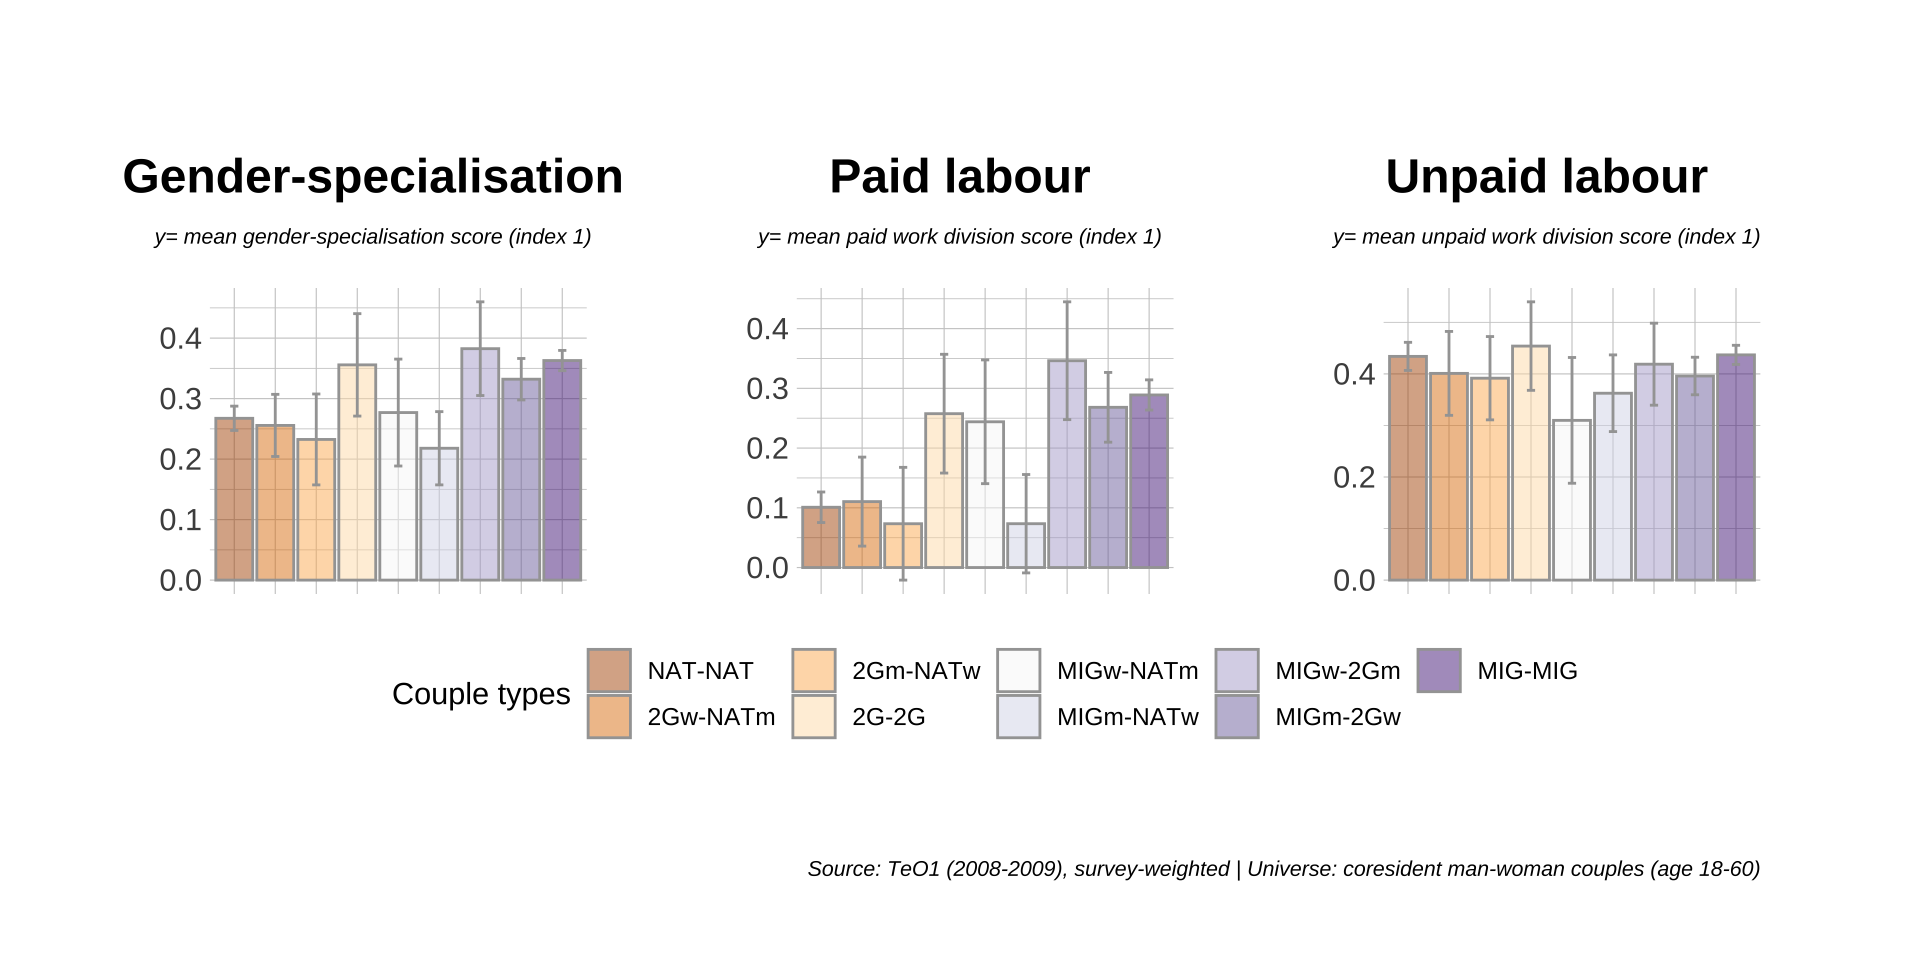
\includegraphics{BSPS-2022-mixed-unions_files/figure-beamer/barplot_gdrspec2FR-1.pdf}
\end{block}

\begin{block}{barplot: sequence by couple type}
\protect\hypertarget{barplot-sequence-by-couple-type}{}
Problem here with gdrm (needs to be defined)

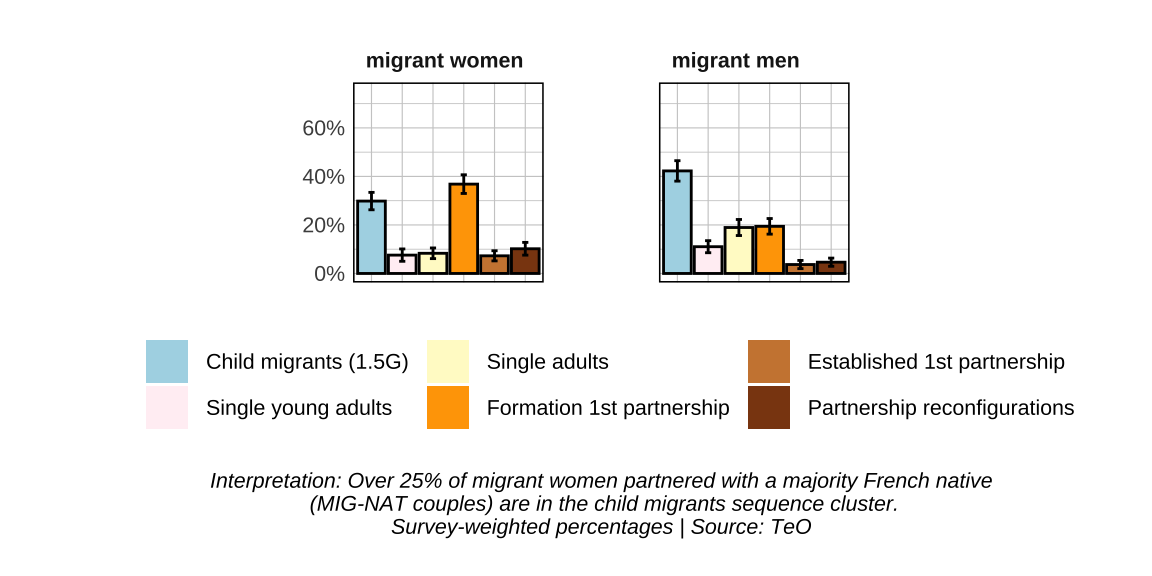
\includegraphics{BSPS-2022-mixed-unions_files/figure-beamer/revbarplot_pam6FR-1.pdf}
\end{block}

\begin{block}{barplots3: joint employment status}
\protect\hypertarget{barplots3-joint-employment-status}{}
\end{block}

\begin{block}{by cpl\_sex}
\protect\hypertarget{by-cpl_sex}{}
\includegraphics{BSPS-2022-mixed-unions_files/figure-beamer/unnamed-chunk-7-1.pdf}
\end{block}

\begin{block}{by regi3}
\protect\hypertarget{by-regi3}{}
\includegraphics{BSPS-2022-mixed-unions_files/figure-beamer/unnamed-chunk-8-1.pdf}
\end{block}

\begin{block}{pam6nat women}
\protect\hypertarget{pam6nat-women}{}
\includegraphics{BSPS-2022-mixed-unions_files/figure-beamer/unnamed-chunk-9-1.pdf}
\end{block}

\begin{block}{Pam6Nat Men}
\protect\hypertarget{pam6nat-men}{}
\includegraphics{BSPS-2022-mixed-unions_files/figure-beamer/unnamed-chunk-10-1.pdf}
\end{block}

\begin{block}{Pam6Nat2 women}
\protect\hypertarget{pam6nat2-women}{}
\includegraphics{BSPS-2022-mixed-unions_files/figure-beamer/unnamed-chunk-11-1.pdf}
\end{block}

\begin{block}{Pam6Nat2 Men}
\protect\hypertarget{pam6nat2-men}{}
\includegraphics{BSPS-2022-mixed-unions_files/figure-beamer/unnamed-chunk-12-1.pdf}
\end{block}
\end{frame}

\begin{frame}[fragile]{Results}
\protect\hypertarget{results-1}{}
\begin{block}{Slides with plot}
\protect\hypertarget{slides-with-plot}{}
\begin{Shaded}
\begin{Highlighting}[]
\FunctionTok{hist}\NormalTok{(cars}\SpecialCharTok{$}\NormalTok{speed)}
\end{Highlighting}
\end{Shaded}

\includegraphics{BSPS-2022-mixed-unions_files/figure-beamer/unnamed-chunk-13-1.pdf}
\end{block}

\begin{block}{Migrant women}
\protect\hypertarget{migrant-women}{}
\note{\begin{figure}

{\centering 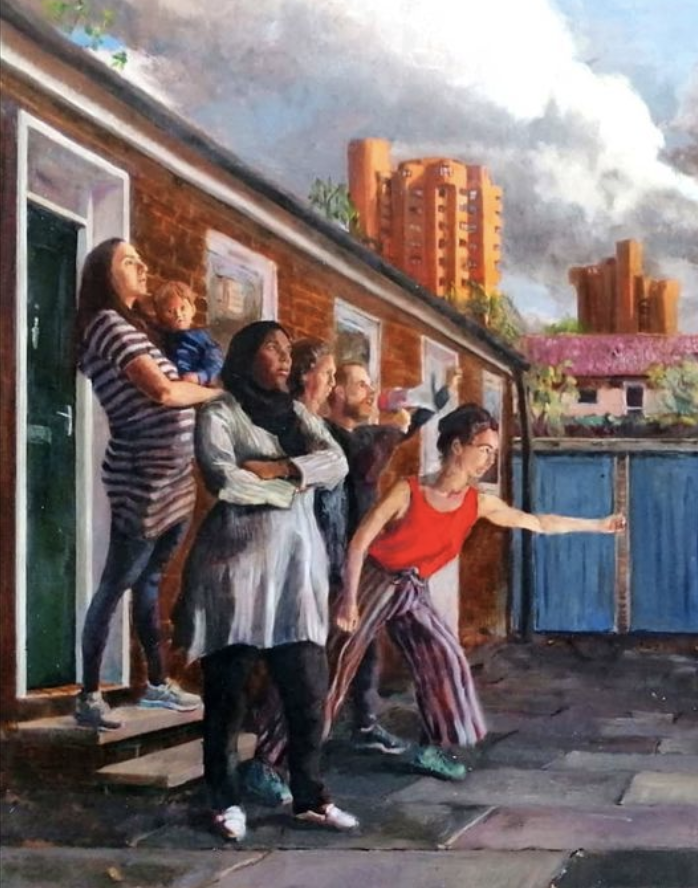
\includegraphics[width=8cm,height=\textheight]{graphics/NicholasBaldion_Eviction.png}

}

\caption{``Nicholas Baldion, Painting of an eviction''}

\end{figure}}
\end{block}
\end{frame}

\begin{frame}{Conclusion}
\protect\hypertarget{conclusion}{}
\begin{itemize}
\tightlist
\item
  Mixed couples are associated with specific and singularly gendered
  trajectories of migration/couple formation: \emph{gendered paths to
  mixing}
\item
  Overall migrants who migrate before family formation seem much more
  likely to form mixed unions (logical)

  \begin{itemize}
  \tightlist
  \item
    For men, it's especially true if they migrated as children
  \item
    For women, it's especially true if they migrated as single adults
  \end{itemize}
\item
  but independent adult migration is mostly accessible to certain origin
  groups, and is overall less accessible to women (lower educational
  level, more resistance to women migrating alone)
\item
  Couple-forming and marriage migration involve majority British and
  French men, and not only migrants or descendants of migrants
  (so-called ``chain migration'')
\item
  Different trajectories of migration/couple formation are associated
  with different outcomes of migration: labour market performance and
  gender-specialisation in couples.
\end{itemize}
\end{frame}



\end{document}
